\documentclass[a4paper,zihao=5]{ctexart}

% ---- 字体与页面 ----
\setmainfont{Times New Roman}
\setsansfont{Arial}
\setmonofont{Consolas}[Scale=0.85]
\usepackage[top=2.5cm,bottom=2.5cm,left=2.5cm,right=2.5cm]{geometry}
\linespread{1.12}

% ---- 数学、图片、表格 ----
\usepackage{amsmath,amssymb}
\usepackage{graphicx}
\usepackage{float}
\usepackage{subcaption}
\usepackage{booktabs}
\usepackage{array}
\usepackage{enumitem}
\usepackage{siunitx}
\usepackage{tikz}
\usetikzlibrary{arrows.meta,positioning,shapes.geometric}

% ---- 顶刊风格低饱和配色 ----
\usepackage{xcolor}
\definecolor{paperblue}{HTML}{21629B}
\definecolor{paperred}{HTML}{BC5040}
\definecolor{papergreen}{HTML}{348070}
\definecolor{papergray}{HTML}{6B7280}
\definecolor{paperlight}{HTML}{F6F8FA}
\definecolor{paperline}{HTML}{D9DEE5}
\definecolor{paperink}{HTML}{23272A}

% ---- 代码 ----
\usepackage{listings}
\lstset{
  language=C++,
  basicstyle=\small\ttfamily,
  keywordstyle=\color{paperblue}\bfseries,
  commentstyle=\color{papergreen},
  stringstyle=\color{paperred},
  numbers=left,
  numberstyle=\tiny\color{papergray},
  numbersep=6pt,
  breaklines=true,
  frame=single,
  rulecolor=\color{paperline},
  tabsize=4,
  showstringspaces=false,
  columns=fullflexible
}

\usepackage[colorlinks=true,linkcolor=paperblue,urlcolor=paperblue,citecolor=paperblue]{hyperref}

\title{\LARGE\textbf{实验三：LZW 编解码实验}}
\author{姓名：梁信、高居博、赵夕涵、刘嘉乐、黎玥含、赵欣瑶、罗雅丹、蓝浩宇\\[2pt]
\normalsize 第5组}
\date{}

\begin{document}
\maketitle

%=====================================================
\section*{一、实验目标}
\addcontentsline{toc}{section}{一、实验目标}
%=====================================================

本实验以 8 位灰度图像 \texttt{b8gray.bmp} 为输入，完成基于 LZW（Lempel--Ziv--Welch）的无损图像编解码。实验目标如下：

\begin{enumerate}[itemsep=2pt]
  \item 理解 LZW 字典编码的基本思想，掌握由像素序列生成压缩码流的方法；
  \item 编写编码程序，以原灰度图像 $I_s$ 为输入，输出压缩文件 \texttt{C.dat}；
  \item 编写解码程序，以 \texttt{C.dat} 为输入，恢复解码图像 $I_d$；
  \item 计算编码后的 bpp 值和原灰度图像的信息熵；
  \item 对 $I_s$ 与 $I_d$ 进行逐像素比较，验证 LZW 编解码的无损性。
\end{enumerate}

%=====================================================
\section*{二、实验原理}
\addcontentsline{toc}{section}{二、实验原理}
%=====================================================

\subsection*{2.1\quad LZW 编码思想}

LZW 是一种典型的自适应字典压缩算法。对于 8 位灰度图像，初始字典包含全部单字节灰度值：
\begin{equation}
  \mathcal{D}_0 = \{0,1,2,\ldots,255\}.
\end{equation}
编码时按行扫描图像像素，持续寻找字典中已经出现的最长序列 $w$。若新序列 $w+k$ 尚未出现在字典中，则输出 $w$ 的编码，并将 $w+k$ 加入字典。随着编码进行，重复纹理、相邻灰度结构和局部模式会被更长的字典项表示，从而减少码字数量。

\subsection*{2.2\quad LZW 解码思想}

解码端采用与编码端相同的初始字典，并根据接收到的码字同步重建字典。设上一条解码序列为 $w$，当前码字对应序列为 $s$，则每读取一个新码字后，把
\begin{equation}
  w + \mathrm{first}(s)
\end{equation}
加入字典。对于 LZW 中常见的特殊情形，即当前码字刚好等于下一条待加入的字典索引，解码序列取为
\begin{equation}
  s = w + \mathrm{first}(w).
\end{equation}
只要编码和解码的字典更新规则一致，最终恢复的像素序列应与原图完全相同。

\subsection*{2.3\quad bpp 与熵}

编码后每像素比特数（bits per pixel, bpp）用于衡量压缩表示的平均码长。本文同时给出仅统计 LZW 码流的 bpp 和包含文件头、调色板等元数据的 \texttt{C.dat} 文件 bpp：
\begin{equation}
  \mathrm{bpp}_{\mathrm{code}} =
  \frac{N_{\mathrm{code}}\times 16}{W\times H},
  \qquad
  \mathrm{bpp}_{\mathrm{file}} =
  \frac{8\times \mathrm{size}(\texttt{C.dat})}{W\times H}.
\end{equation}

原灰度图像的信息熵定义为
\begin{equation}
  H(I_s) = -\sum_{k=0}^{255} p_k \log_2 p_k,
\end{equation}
其中 $p_k$ 表示灰度级 $k$ 在原图中的出现概率。熵反映图像灰度分布的不确定性，是无损编码平均码长的重要参考下界。

%=====================================================
\section*{三、方法描述}
\addcontentsline{toc}{section}{三、方法描述}
%=====================================================

\subsection*{3.1\quad 编码框图}

\begin{figure}[H]
\centering
\resizebox{\textwidth}{!}{%
\begin{tikzpicture}[
  node distance=8mm and 11mm,
  box/.style={draw=paperline, fill=paperlight, rounded corners=2pt, align=center, minimum height=8mm, text width=32mm},
  decision/.style={diamond, draw=paperblue, fill=paperblue!7, aspect=2.1, align=center, inner sep=1pt, text width=28mm},
  arrow/.style={-{Latex[length=2.2mm]}, thick, color=paperblue}
]
\node[box] (a) {读入 $I_s$\\\texttt{b8gray.bmp}};
\node[box, right=of a] (b) {按行提取\\灰度像素序列};
\node[box, right=of b] (c) {初始化字典\\0--255};
\node[decision, below=of c] (d) {$w+k$\\是否在字典中};
\node[box, left=of d] (e) {是：扩展\\当前序列 $w$};
\node[box, right=of d] (f) {否：输出\\$w$ 的编码};
\node[box, below=of f] (g) {加入新字典项\\$w+k$};
\node[box, below=of d] (h) {更新 $w=k$\\继续扫描};
\node[box, below=of h] (i) {输出末尾码字\\写入 \texttt{C.dat}};
\draw[arrow] (a) -- (b);
\draw[arrow] (b) -- (c);
\draw[arrow] (c) -- (d);
\draw[arrow] (d) -- (e);
\draw[arrow] (e.south) |- ++(0,-5mm) -| (d.south);
\draw[arrow] (d) -- (f);
\draw[arrow] (f) -- (g);
\draw[arrow] (g) -- (h);
\draw[arrow] (h) -- (i);
\end{tikzpicture}%
}
\caption{LZW 编码流程图}
\end{figure}

\subsection*{3.2\quad 编码代码}

编码程序位于 \texttt{Task3/main.cpp}。核心函数包括：
\begin{itemize}[itemsep=2pt]
  \item \texttt{GetImageBytes}：从 \texttt{HXLBMPFILE} 中提取 8 位灰度像素序列；
  \item \texttt{LzwEncode}：按照 LZW 字典规则输出 16 bit 码流；
  \item \texttt{SaveCompressedFile}：将图像尺寸、调色板、码流数量和码字写入 \texttt{C.dat}；
  \item \texttt{CalculateEntropy}：统计原图灰度概率并计算信息熵。
\end{itemize}

\subsection*{3.3\quad 解码框图}

\begin{figure}[H]
\centering
\resizebox{\textwidth}{!}{%
\begin{tikzpicture}[
  node distance=8mm and 10mm,
  box/.style={draw=paperline, fill=paperlight, rounded corners=2pt, align=center, minimum height=8mm, text width=34mm},
  decision/.style={diamond, draw=papergreen, fill=papergreen!7, aspect=2.0, align=center, inner sep=1pt, text width=28mm},
  arrow/.style={-{Latex[length=2.2mm]}, thick, color=papergreen}
]
\node[box] (a) {读入压缩文件\\\texttt{C.dat}};
\node[box, right=of a] (b) {读取图像信息\\调色板和码流};
\node[box, right=of b] (c) {初始化字典\\0--255};
\node[box, below=of c] (d) {读取首码字\\输出首序列};
\node[decision, left=of d] (e) {当前码字\\是否已在字典中};
\node[box, below=of e] (f) {恢复当前序列\\或处理特殊情形};
\node[box, right=of f] (g) {加入字典项\\$w+\mathrm{first}(s)$};
\node[box, right=of g] (h) {输出像素序列\\重建 $I_d$};
\node[box, below=of h] (i) {保存 \texttt{Id.bmp}\\并与 $I_s$ 比较};
\draw[arrow] (a) -- (b);
\draw[arrow] (b) -- (c);
\draw[arrow] (c) -- (d);
\draw[arrow] (d) -- (e);
\draw[arrow] (e) -- (f);
\draw[arrow] (f) -- (g);
\draw[arrow] (g) -- (h);
\draw[arrow] (h) -- (i);
\end{tikzpicture}%
}
\caption{LZW 解码流程图}
\end{figure}

\subsection*{3.4\quad 解码代码}

解码程序同样位于 \texttt{Task3/main.cpp}。核心函数包括：
\begin{itemize}[itemsep=2pt]
  \item \texttt{LoadCompressedFile}：读取 \texttt{C.dat} 中保存的图像元数据、调色板和 LZW 码流；
  \item \texttt{LzwDecode}：按 LZW 解码规则恢复原始像素序列；
  \item \texttt{PutImageBytes}：将解码像素写回 \texttt{HXLBMPFILE} 图像对象；
  \item \texttt{SameImage}：比较原图和解码图的尺寸、通道数及全部像素值。
\end{itemize}

%=====================================================
\section*{四、实验结果}
\addcontentsline{toc}{section}{四、实验结果}
%=====================================================

\subsection*{4.1\quad 图像恢复结果}

\begin{figure}[H]
  \centering
  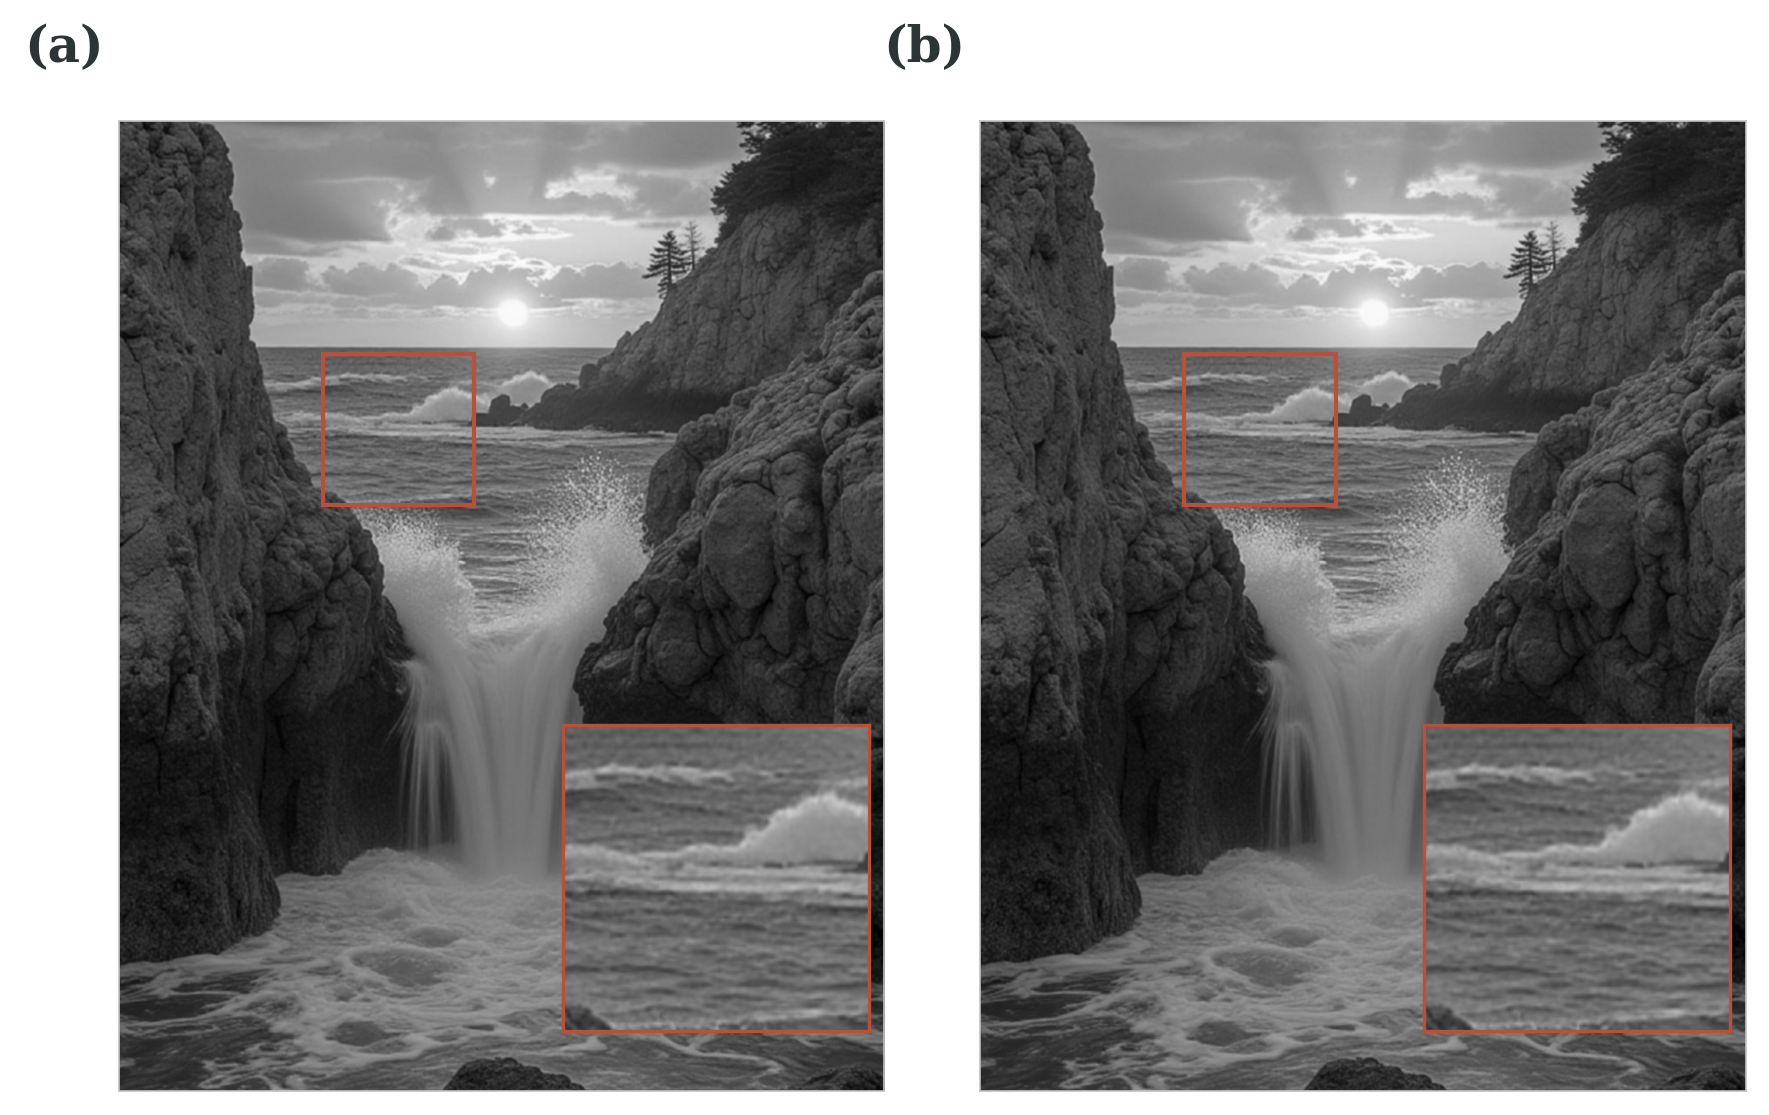
\includegraphics[width=0.96\textwidth]{figures/fig_input_decoded.png}
  \caption{(a) 原图 $I_s$（\texttt{b8gray.bmp}）与 (b) 由 \texttt{C.dat} 解码得到的图像 $I_d$。红色矩形区域为放大对比细节。}
\end{figure}

从视觉上看，解码图像与原图完全一致。进一步对局部细节区域进行逐像素验证（图~\ref{fig:diff}），差分像素数为 0（$\Delta=0$），证实本实验 LZW 编解码为严格无损恢复。

\begin{figure}[H]
  \centering
  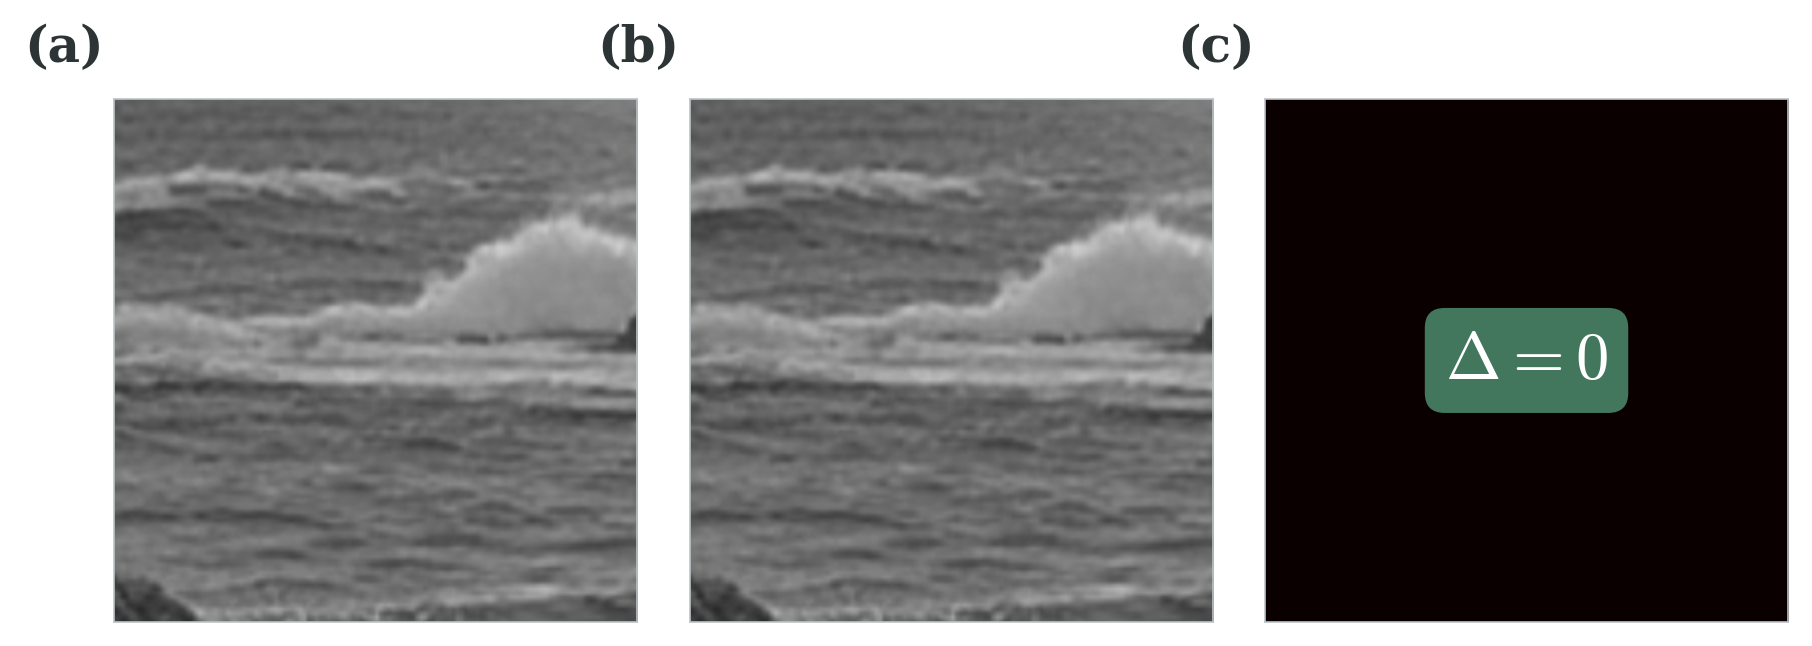
\includegraphics[width=0.96\textwidth]{figures/fig_difference.png}
  \caption{局部细节放大对比：(a)~原图 $I_s$ 裁剪区域，(b)~解码图 $I_d$ 同一区域，(c)~逐像素差分 $|I_s-I_d|$，$\Delta=0$ 表明完全无损。}
  \label{fig:diff}
\end{figure}

\subsection*{4.2\quad 原图灰度分布}

\begin{figure}[H]
  \centering
  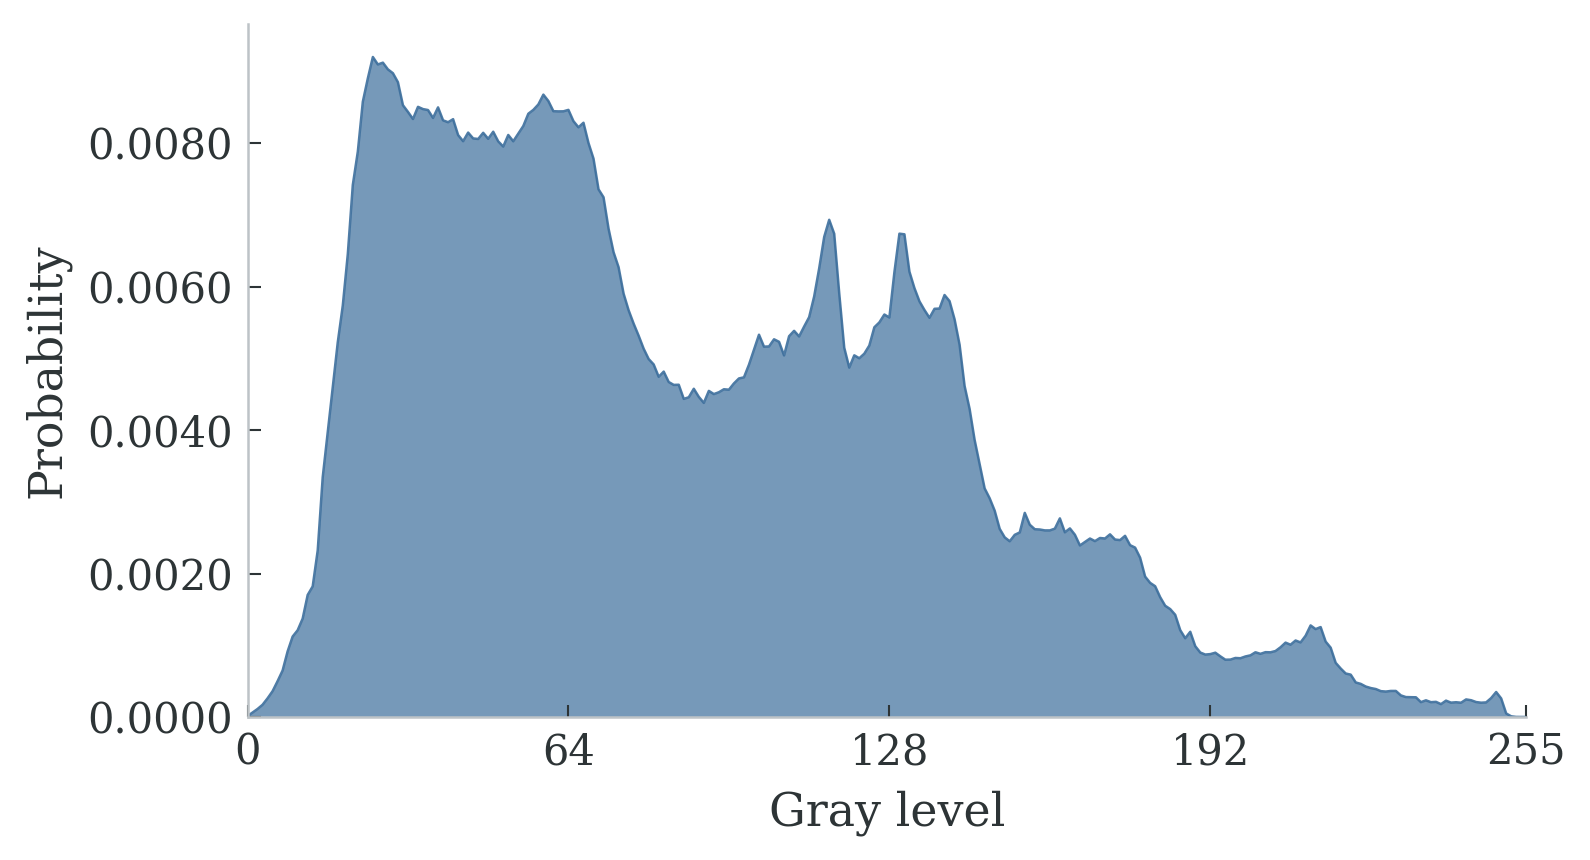
\includegraphics[width=0.80\textwidth]{figures/fig_histogram_source.png}
  \caption{原图 $I_s$ 的归一化灰度直方图}
\end{figure}

原图灰度主要集中在中低灰度区间，同时覆盖了较宽的灰度范围。该分布决定了图像熵较高，但局部像素序列仍存在可被 LZW 字典利用的重复结构。

\subsection*{4.3\quad bpp、熵与同一性验证}

\begin{figure}[H]
  \centering
  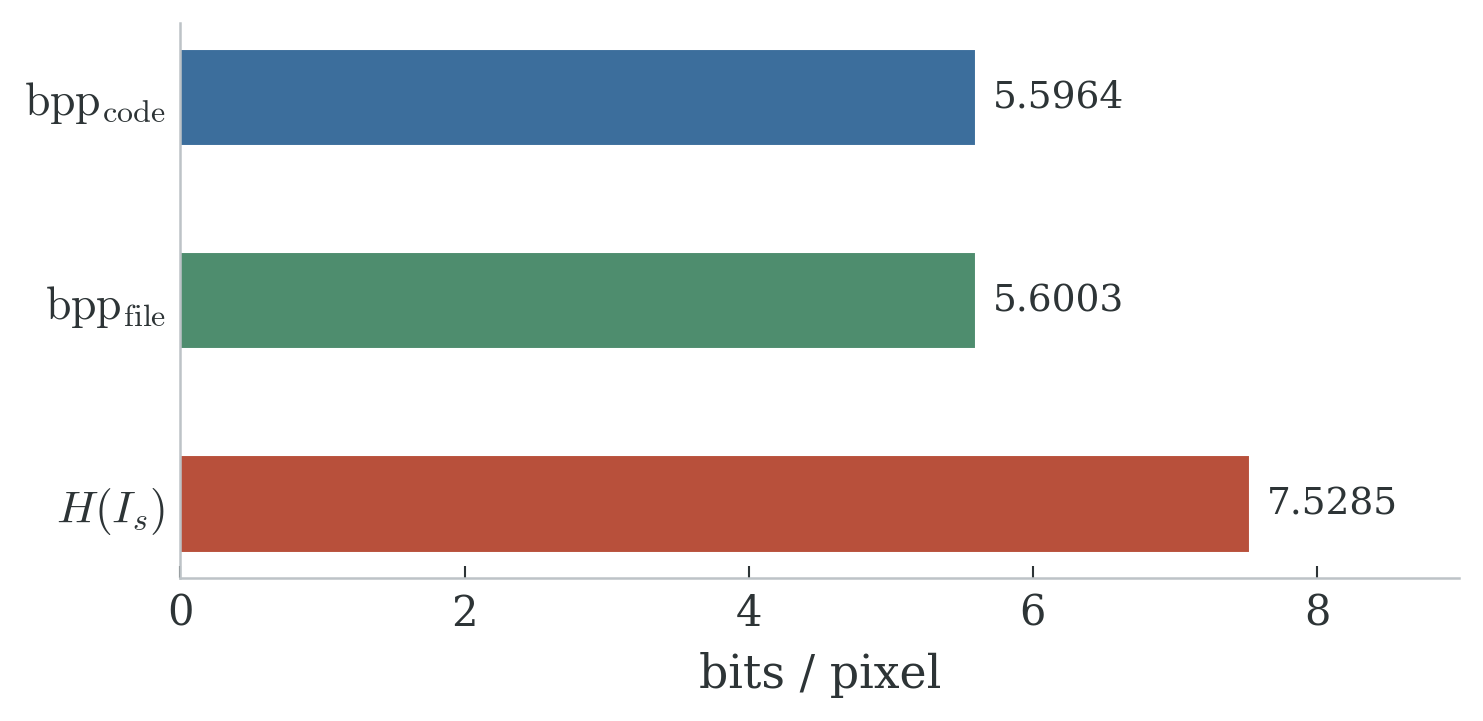
\includegraphics[width=0.78\textwidth]{figures/fig_metrics.png}
  \caption{LZW 编码 bpp 与原图信息熵 $H(I_s)$ 对比。$\mathrm{bpp_{code}}$ 和 $\mathrm{bpp_{file}}$ 均低于信息熵，说明 LZW 字典有效利用了像素序列的冗余。}
\end{figure}

\begin{table}[H]
\centering
\begin{tabular}{ll}
\toprule
\textbf{项目} & \textbf{结果} \\
\midrule
输入图像 & \texttt{b8gray.bmp} \\
图像尺寸 & $1314 \times 1666$ \\
原始像素数 & $2{,}189{,}124$ \\
LZW 码字数量 & $765{,}705$ \\
编码后 bpp（仅 LZW 码流） & $5.596430$ bit/pixel \\
编码后 bpp（包含 \texttt{C.dat} 文件头） & $5.600275$ bit/pixel \\
原灰度图像熵 & $7.528544$ bit/pixel \\
$I_s$ 与 $I_d$ 是否相同 & YES \\
\bottomrule
\end{tabular}
\caption{实验三运行结果汇总}
\end{table}

\subsection*{4.4\quad 输出文件}

\begin{table}[H]
\centering
\begin{tabular}{lll}
\toprule
\textbf{文件} & \textbf{类型} & \textbf{说明} \\
\midrule
\texttt{C.dat} & 压缩文件 & 编码程序输出，包含图像元数据、调色板与 LZW 码流 \\
\texttt{Id.bmp} & 解码图像 & 解码程序由 \texttt{C.dat} 恢复得到 \\
\texttt{result.txt} & 文本结果 & 保存 bpp、熵和同一性验证结果 \\
\texttt{figures/*.png} & 报告图片 & 报告中插入的图像、直方图和指标图 \\
\bottomrule
\end{tabular}
\caption{实验输出文件说明}
\end{table}

%=====================================================
\section*{五、结论}
\addcontentsline{toc}{section}{五、结论}
%=====================================================

本实验完成了灰度图像的 LZW 编码与解码。程序以 \texttt{b8gray.bmp} 为输入生成 \texttt{C.dat}，再由该压缩文件恢复出 \texttt{Id.bmp}。逐像素比较结果表明 $I_s$ 与 $I_d$ 完全一致，验证了算法实现的无损性。实验测得仅码流 bpp 为 $5.596430$ bit/pixel，包含文件头后的 \texttt{C.dat} bpp 为 $5.600275$ bit/pixel，均低于原图单像素灰度熵 $7.528544$ bit/pixel，说明 LZW 字典有效利用了图像像素序列中的上下文重复结构。

%=====================================================
\section*{六、附录：函数代码}
\addcontentsline{toc}{section}{六、附录}
%=====================================================

以下为除 \texttt{HXLBMPFILE} 类代码外的实验三主要代码。

\lstinputlisting[caption={实验三 LZW 编解码完整实现},label={lst:lzw}]{main.cpp}

\end{document}
